\documentclass[pdftex,a4paper,12pt]{report}
\newtheorem{theorem}{Theorem}[section]
\newtheorem{lemma}[theorem]{Lemma}
\newtheorem{proposition}[theorem]{Proposition}
\newtheorem{corollary}[theorem]{Corollary}

\newenvironment{proof}[1][Proof]{\begin{trivlist}
\item[\hskip \labelsep {\bfseries #1}]}{\end{trivlist}}
\newenvironment{definition}[1][Definition]{\begin{trivlist}
\item[\hskip \labelsep {\bfseries #1}]}{\end{trivlist}}
\newenvironment{example}[1][Example]{\begin{trivlist}
\item[\hskip \labelsep {\bfseries #1}]}{\end{trivlist}}
\newenvironment{remark}[1][Remark]{\begin{trivlist}
\item[\hskip \labelsep {\bfseries #1}]}{\end{trivlist}}

\newcommand{\qed}{\nobreak \ifvmode \relax \else
      \ifdim\lastskip<1.5em \hskip-\lastskip
      \hskip1.5em plus0em minus0.5em \fi \nobreak
      \vrule height0.75em width0.5em depth0.25em\fi}
\def\therefore{
\leavevmode
\lower0.1ex\hbox{$\bullet$}
\kern-0.2em\raise0.7ex\hbox{$\bullet$}
\kern-0.2em\lower0.2ex\hbox{$\bullet$}
\thinspace}
\usepackage[linesnumbered,boxruled,vlined]{algorithm2e}
\usepackage{amsmath}
\usepackage{multicol}
\usepackage{hyperref}
\usepackage{color}
\usepackage{fullpage}
\usepackage{graphicx}
\newcommand{\abs}[1] {$\mid #1 \mid$}
\renewcommand{\thesection}{\arabic{section}}

\hypersetup{
  colorlinks,
  citecolor=blue,
  linkcolor=blue,
  urlcolor=blue
}
\begin{document}
\begin{titlepage}
\begin{center}

\textsc{\LARGE IIT Kanpur}\\[1.5cm]

\textsc{\Large CS345A - AlgorithmsII}\\[0.5cm]

% Title
{ \huge \bfseries Assignment 3 \\[0.4cm] }


\begin{minipage}{0.4\textwidth}
\begin{flushleft} \large
Anjani Kumar\\
11101
\end{flushleft}
\end{minipage}
\begin{minipage}{0.4\textwidth}
\begin{flushright} \large
Sumedh Masulkar\\
11736
\end{flushright}
\end{minipage}

\vfill

% Bottom of the page
{\large February 14, 2014}

\end{center}
\end{titlepage}

\tableofcontents
\newpage


\section{A Job Scheduling Problem}
Consider the following jobs starting from t=$0$:\\
\begin{center}

\begin{tabular}{c|c|c}
\hline
Job & Deadline & Penalty\\
\hline
Job1 & 1 & 1\\
Job2 & 2 & 1\\
Job3 & 3 & 100\\
Job4 & 3 & 100\\
\hline
\end{tabular}

\end{center}
We have to schedule these jobs such that overall penalty is minimum.
\subsection{Strategy 1:}Schedule the jobs in increasing order of deadlines.
\begin{figure}[h]
\centering
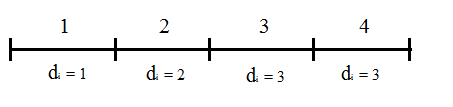
\includegraphics[scale=0.5]{fig1.png}
\caption{Job Schedule for strategy 1}
\label{fig1}
\end{figure}
\begin{itemize}
\item According to this strategy, the jobs would be scheduled as per fig \ref{fig1}.
\item In this case, job 4 exceeds its deadline. Hence total penalty is $P_{4}=100$.
\end{itemize}
\begin{figure}[h]
\centering
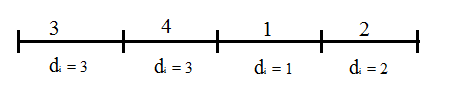
\includegraphics[scale=0.5]{fig2.png}
\caption{A counter-example for strategy 1}
\label{fig2}
\end{figure}
\begin{itemize}
\item In fig \ref{fig2}, jobs 1 and 2 exceed their deadlines. Hence total penalty for this case is $P_{1}+P_{2} = 2$.
\item Since the penalty for fig \ref{fig2} is less than that of fig \ref{fig1}. Therefore Strategy 1 is not optimal.
\end{itemize}
\begin{multicols}{2}
\begin{center}
\begin{itemize}
\item Job schedule according to above strategy
\end{itemize}
\begin{tabular}{c|c|c|c}
\hline
Job & Slot & Deadline & Penalty\\
\hline
Job1 & 0-1 & 1 & 0\\
Job2 & 1-2 & 2 & 0\\
Job3 & 2-3 & 3 & 0\\
Job4 & 3-4 & 3 & 100\\
\hline
\end{tabular}
\end{center}
\setlength{\columnseprule}{0.2pt}
\columnbreak
\begin{center}
\begin{itemize}
\item A Possible Counter-example for above strategy
\end{itemize}
\begin{tabular}{c|c|c|c}
\hline
Job & Slot & Deadline & Penalty\\
\hline
Job3 & 0-1 & 3 & 0\\
Job4 & 1-2 & 3 & 0\\
Job1 & 2-3 & 1 & 1\\
Job2 & 3-4 & 2 & 1\\
\hline
\end{tabular}
\end{center}
\end{multicols}
\newpage
\subsection{Strategy 2:}Schedule the jobs in decreasing order of penalties and while scheduling a job if there is an empty slot
available before its deadline then schedule it as early as possible.
\begin{figure}[h]
\centering
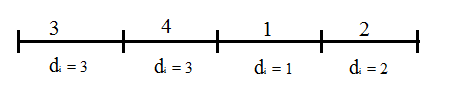
\includegraphics[scale=0.5]{fig2.png}
\caption{Job schedule for strategy 2}
\label{fig3}
\end{figure}
\begin{itemize}
\item According to this strategy, the jobs would be scheduled as per fig\ref{fig3}.
\item In this case, jobs 1 and 2 exceed their deadlines. Hence total penalty is $P_{1} + P_{2} = 2$.
\end{itemize}
\begin{figure}[h]
\centering
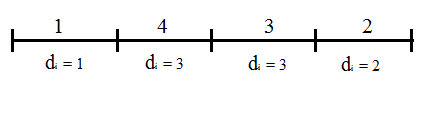
\includegraphics[scale=0.5]{fig3.png}
\caption{A counter example for strategy 2}
\label{fig4}
\end{figure}
\begin{itemize}
\item In fig \ref{fig4}, only job 2 exceeds its deadline. Hence total penalty for this case is $P_{2} = 1$.
\item Since the penalty for fig \ref{fig4} is less than fig \ref{fig3}. Therefore Strategy 2 is not optimal.
\end{itemize}
\begin{multicols}{2}
\begin{center}
\begin{itemize}
\item Job schedule according to above strategy
\end{itemize}
\begin{tabular}{c|c|c|c}
\hline
Job & Slot & Deadline & Penalty\\
\hline
Job3 & 0-1 & 3 & 0\\
Job4 & 1-2 & 3 & 0\\
Job1 & 2-3 & 1 & 1\\
Job2 & 3-4 & 2 & 1\\
\hline
\end{tabular}
\end{center}

\setlength{\columnseprule}{0.2pt}
\columnbreak
\begin{center}
\begin{itemize}
\item A Possible Counter-example for above strategy
\end{itemize}
\begin{tabular}{c|c|c|c}
\hline
Job & Slot & Deadline & Penalty\\
\hline
Job1 & 0-1 & 1 & 0\\
Job4 & 1-2 & 3 & 0\\
Job3 & 2-3 & 3 & 0\\
Job2 & 3-4 & 2 & 1\\
\hline
\end{tabular}
\end{center}
\end{multicols}
\subsection{Strategy 3:}schedule the jobs in decreasing order of penalties and while scheduling a job if there is an empty time
slot available before its deadline, then schedule it to the latest such slot.
\subsubsection{Data Structure Used:}
\begin{itemize}
\item Let the number of jobs be n.
\item An array (Temp) of size n, which after sorting, contains the index of jobs according to non-increasing order of their penalty.
\item A complete Binary search tree (T) of size n, used to store the available slots. Such that, on an in-order traversal of T, the slots are printed in an ascending order (1,2,...n).\label{tree}
\item An array (Opt) of size n, which contains the optimal job schedule.
\item An array (flag) of size n. flag[\emph{j}] = 1, if the deadline of job in $Temp[j]$ has been exceeded. Otherwise it is 0.
\item index of all the arrays start from 1.
\end{itemize}
\subsubsection{Brief description:}
\begin{itemize}
\item The jobs are taken one by one (according to decreasing order of their penalty) from the array $Temp$ (from index 1 to n). Let the job corresponding to current element $i$ be $j$. The deadline corresponding to $j$ is found. Let it be \emph{$d_{j}$}.
\item A node with value same as that of the \emph{$d_{j}$} is searched in T. Following cases are possible:
\begin{enumerate}
\item Case1: The Node is present in T.
\begin{itemize}
\item The corresponding node is deleted from T.
\item The value of Opt[\emph{$d_{j}$}] is updated to $j$
\end{itemize}
\item Case2: The Node is absent and its predecessor is present in T.
\begin{itemize}
\item Predecessor(\emph{$d_{j}$}) in tree T is calculated. Let it be \emph{$p_{j}$}.
\item The corresponding predecessor node is deleted.
\item The value of Opt[\emph{$p_{j}$}] is updated to $j$.
\end{itemize}
\item Case3: The Node is absent and its predecessor does not exist in T.
\begin{itemize}
\item In this case, Predecessor(\emph{$d_{j}$}) returns value -1.
\item This implies that the job's deadline has been exceeded.
\item The value of flag[\emph{i}] is switched from 0 to 1.
\end{itemize}
\end{enumerate}
\item After the array $Temp$ is traversed completely:
\begin{itemize}
\item The jobs with high flag are appended to array $Opt$ in the end. 
\item The array \emph{Opt} is returned.
\end{itemize}

\end{itemize}
\subsection{Functions used:}
\begin{itemize}
\item \textbf{Sort}($Temp$):
Sorts the passed array $Temp$(which contains the jobs) in non-increasing order of their penalties.
\item \textbf{Search}(T, $V$):
Searches for the node with value $V$ in tree T and returns $TRUE$ if found, else it returns $FALSE$.
\item\textbf{Predecessor}($Node$):
Return the value of predecessor of $Node$ if it is present, otherwise it returns $-1$.
\end{itemize}
\newpage
\subsection{Pseudo Code}
        \begin{algorithm}

        Job\_Scheduler($J$)\{\\
        \Begin{
                Initialize arrays $Temp$, $Opt$, $flag$ of size \textbf{$n$}.\\
                \textbf{Sort}(Temp);\makebox[40pt]{}\textcolor{blue}{//Sorts array of jobs in
decreasing order of penalties}\\
                $T$ $\gets$ A complete binary tree of size $n$ as described in section \ref{tree}.\\
                found $\gets$ false\;
                $i$ $\gets$ 1;\makebox[40pt]{}\textcolor{blue}{//$i$ keeps note of number of slots filled
in Opt.}\\
                \For{$j\ \gets$ 1 to $n$}{ \makebox[80pt]{}\textcolor{green}{//$O(n\
log(n))$.}\\
                        found $\gets$ \textbf{Search}($T$, Temp[j]$\rightarrow$deadline)\;
                        \eIf{found==true}{
                                Opt[Temp[j]$\rightarrow$deadline] $\gets$ Temp[j]\;
                                $i++$\;
                                \textbf{Delete}($T$, Temp[j]$\rightarrow$deadline)\;
                                found $\gets$ false\;
                        }{
                                pred $\gets$ \textbf{Predecessor}(Temp[j]$\rightarrow$deadline)\;
                                \eIf{pred$<>$-1}{
                                        Opt[pred] $\gets$ Temp[j]\;
                                        $i++$\;
                                        \textbf{Delete}($T$, pred)\;
                                }{
                                        flag[j] = 1\;
                                }
                        }
                }
                \For{$j\ \gets$ 1 to $n$}{
                        \If{flag[j]$<>$0}{
                                Opt[i] $\gets$ Temp[j]\;
                                $i++$\;
                        }
                }
                return $Opt$\;
        }
        \}\\
        \caption{Pseudo code for Job\_Scheduler($J$)}

        \end{algorithm}
\subsection{Time Complexity}
\begin{itemize}
\item It takes $O(n)$ time to build the tree $T$.
\item \textbf{Sort} takes $O$(n log $n$) time, where $n$ is the number of jobs.
\item The functions \textbf{Search},\textbf{Delete} and \textbf{Predecessor} takes $O$(log $k$) time, where $k$ is the size of the tree T at any given time. 
\item Traversing the arrays $flag$ and $Opt$ takes $O$($n$) time.
\item As shown in the Pseudo code, overall the algorithm takes  \textbf{$O$(nlog $n$)} time.
\end{itemize}
\subsection{Proof Of Correctness}
Let J = $j_{1},j_{2},...j_{n}$ be $n$ jobs in increasing order of penalty.
\begin{lemma}
\mbox{}
\label{lemma}
\begin{center}

In the optimal solution $Opt(J)$, $j_{n}$ must be scheduled at or before its deadline.

\end{center}
\end{lemma}
\begin{proof}
\mbox{}\\
{Proof by Contradiction:}\\
Let us assume that lemma \ref{lemma} is false. Therefore $\exists$ an optimal solution $Opt(j')$ s.t. $j_{n}$ is scheduled after its deadline. Let $j_{i}$ be the job replaced by $j_{n}$ in the optimal solution.
\begin{equation}
Opt(j') = Opt(j)+Penalty(\texttt{$j_{n}$}) - Penalty(\texttt{$j_{i}$})\\
\end{equation}
\begin{equation}
Penalty(\texttt{$j_{n}$}) - Penalty(\texttt{$j_{i}$}) \geq 0 \\
\end{equation}
\begin{equation}
\Rightarrow Opt(j')\geq Opt(j)\\
\end{equation}
Therefore, $Opt(j')$ is not the optimal solution. Hence our assumption was wrong.\\
Hence Proved.
\end{proof}
Let J = $j_{1},j_{2},...j_{n}$ be $n$ jobs in increasing order of penalty.\\
Let J' = J/$j_{n}$\\

\begin{theorem}
\label{theorem}
$Opt(J) = Opt(J')+Penalty(j_{n})$
\end{theorem}
\begin{proof}
\mbox{}\\
\begin{itemize}
\item Part A:
\\ When we have $Opt{J'}$ and $j_{n}$ is to be scheduled. Following cases are possible:\\
%\begin{align*}
Penalty($j_{n}$) = 
					$\begin{cases}
					0 \makebox[100pt]{}\textbf{if $j_{n}$ is scheduled within its deadline}\\
					\texttt{$P_{j_{n}}$} \makebox[90pt]{}\textbf{if $j_{n}$ is scheduled outside its deadline}\\
					\end{cases}$
					\\
%\end{align*}
\begin{equation}
\label{eq1}
\Rightarrow Opt(J) \leq Opt(J') + Penalty(j_{n})
\end{equation}
\item Part B:\\
 When we have $Opt(J)$, using lemma \ref{lemma}, we can say that job $j_{n}$ will be scheduled on or before its deadline.\\
\begin{equation}
\label{eq2}
 \Rightarrow Opt(J') \leq Opt(J) - Penalty(j_{n})
\end{equation} 
\end{itemize}
\begin{equation}
\ref{eq1} \& \ref{eq2} \Rightarrow Opt(J) = Opt(J')+Penalty(j_{n})
\end{equation}
\end{proof}
\begin{itemize}
\item The algorithm stops only when entire array $Temp$(which contains all jobs) is traversed. Therefore all the jobs are scheduled.
\item The algorithm schedules the jobs with higher penalty in vacant slots that are closest to their deadlines (from the left side).
\item So at any given step say $i$, $Opt(J_{i})$ is kept as low as possible. Since the jobs are added in a non increasing order of their penalties, future optimum values would also be minimum. Hence $Opt(J)$ is minimum for this strategy. 
\end{itemize}
\subsection{Space Complexity}
\begin{itemize}
\item Arrays- $Temp$, $Opt$ and $flag$ take $O(n)$ space.
\item Tree $T$ takes $O(n)$ space.
\end{itemize}
\begin{center}
Overall Space complexity = $O(n)$
\end{center}
\newpage


\section{Hierarchical Metric}
	\subsection{Description}
	Given a set of points $P$ = \{$p_1,\ p_2,\ \ldots, \ p_n$\}, with distance function $d$ on the
	set $P$.\\
	
	We need to build a hierarchical metric on $P$ that is constructed as follows:
	\begin{itemize}
		\item
		We build a rooted tree $T$ with n leaves, and associate with each node $v$ of $T$, 
		and $h(v)$. Value of $h(v)$ should be such that
			\begin{itemize}
				\item $h(v)$ = 0, for each leaf.
				\item If $u$ is parent of $v$ in $T$, then $h(u) \geq  h(v) $.
			\end{itemize}
		\item
		For any pair of points $p_i$ \& $p_j$, their distance $\tau (p_i,\ p_j)$ is defined as:
		We determine the lowest common ancestor $v$ in $T$ of the leaves containing $p_i$ and 
		$p_j$, and define $\tau (p_i,\ p_j)$ = $h(v)$.
		\item
		We say that a \emph{hierarchical metric} $\tau$ is consistent with our distance function
		$d$, if for all pairs ($p_i$, $p_j$), we have $\tau(p_i,\ p_j)\ \leq\ d(p_i,\ p_j)$.
		\item
		Given a polynomial time algorithm that takes the distance function $d$ and produces
		a \emph{hierarchical metric} $\tau$ with the following properties:
			\begin{enumerate}
				\item
				$\tau$ is consistent with $d$, and
				\item
				If $\tau$' is any other hierarchical metric constant with $d$, then $\tau$'($p_i,\ p_j$) $\leq\ \tau(p_i,\ p_j)$ 
				for each pair of points $p_i$ and $p_j$.
			\end{enumerate}
	\end{itemize}

	\subsection{Approach}
	\begin{itemize}
		\item
		First of all, we shall sort the pair of points according to their distances in non-decreasing order. The size of array to sort shall
		be the number of pairs $i.e.,$ $n \choose 2$. Thus, the array will be an array of structures, where is structure keeps $p_i$, $p_j$, and 
		$d(p_i,\ p_j)$. And sorting will be done using $d(p_i,\ p_j)$ as key. The \textbf{Sort(D)} function does this, in $O(n^2\ log(n))$ time.
		\item
		For the nearest pair ($p_i,\ p_j$), we take an empty rooted tree $T$, with value of root as $d(p_i,\ p_j)$ and children as $p_i$ and $p_j$. 
		\item
		Now to insert the next pair of points ($p_i,\ p_j$), there are three cases possible.
			\item \textbf{\underline{Case 1:}}
			$p_i$ and $p_j$ both have already been added to the tree $T$.
				\begin{itemize}
					\item This doesn't require us to do anything.
				\end{itemize}
			\item \textbf{\underline{Case 2:}}
			$p_i$ and $p_j$ both have not been added to the tree $T$.
				\begin{itemize}
					\item Create a new node \textbf{$temp$}, with value $d(p_i,\ p_j)$ and children as nodes containing $p_i$ and $p_j$.
					\item Create a new root, with left child as the old root, and right child as $temp$ created above. The value of new root will 
					be the maximum of its child $i.e.,$ value of $temp$, since value of root must be less than equal to value of $temp$.
				\end{itemize}
			\item \textbf{\underline{Case 3:}}
			Among $p_i$ and $p_j$, one has been added to the tree $T$.
			\\\\Let the node already added be $p_x$ and the other be $p_y$.
				\begin{itemize}
					\item $\tau(x,\ y)$ for any pair of points($x,\ y$) already added to the tree will definitely be smaller than $d(p_i,\ p_j)$.
					\item Create a new root, with left child as the old root, and right child as node containing $p_y$. The value of this new
					root, $i.e., \tau$ will be $d(p_i,\ p_j)$.
				\end{itemize}
			\item An array $V$ of size $n$ can do the job of searching a point in a tree using $O(1)$ time and $O(n)$ space. If the point $p_i$ has been 
			inserted in the tree $T$, we set $V[i]$ = 1, else $V[i]$ = 0.
	\end{itemize}
	We claim that tree $T$ such formed is the \emph{hierarchical metric} for given ($P, d$).
	\subsection{Pseudo Code}
	\begin{algorithm}	
	Hierarchical\_Metric($P$, $d$)\{\\
	\Begin{
		Declare an empty array $D$ of structures of size \textbf{$^nC_2$}.\\
		$k\ \gets$ 0; $n\ \gets$ \abs{P}\;
		\For{$i\ \gets$ 1 to $n$}{ \makebox[80pt]{}\textcolor{green}{//$O(n^2)$.}\\
			\For{$j\ \gets$ $i$ to $n$}{
				$D(k)\rightarrow d\ =$ $d(p_i,\ p_j)$;
				$D(k)\rightarrow points\ =$ $(p_i,\ p_j)$\;
				$k++$\;
			}
		}
		\textbf{Sort}(D);
		 \makebox[40pt]{}\textcolor{green}{//$O(n^2\ log(n))$.}
		 \makebox[10pt]{} \textcolor{blue}{//Using $d$ as key to compare.}\\
		Initialize an empty array $V$ of size $n$\;
		Create a tree $T$ rooted at $root$\;
		$(p_i,\ p_j)\ = D(0)\rightarrow points$\;
		root$\rightarrow$val = $d(p_i,\ p_j)$\;
		create new leaves(children \textcolor{red}{NULL}) templeft, tempright\;
		templeft$\rightarrow$val = $p_i$;
		tempright$\rightarrow$val = $p_j$\;
		root$\rightarrow$left = templeft;
		root$\rightarrow$right = tempright\;
      	$V[i]$ $\gets$ 1; $V[j]$ $\gets$ 1\; 
		\For{$k\gets $ 1 to $^n C_2$}{\makebox[10pt]{}\textcolor{green}{//$O(n^2)$.}
			\makebox[20pt]{} \textcolor{blue}{//$O(1)$ for search, iterating over $O(n^2)$ items of array.}\\
			$(p_i,\ p_j)\ = D(k)\rightarrow points$\;
			\uIf{$V[i]$==1 \& $V[j]$==1}{
 				\textcolor{blue}{/*Ignore*/}; \makebox[80pt]{}\textcolor{green}{//$O(1)$.}\\
    		}
      		\uElseIf{$V[i]$==0 \& $V[j]$==0}{
      			create new nodes $newroot,\ temp,$\;
      			create new leaves(children \textcolor{red}{NULL}) templeft, tempright\;
      			templeft$\rightarrow$val = $p_i$;
      			tempright$\rightarrow$val = $p_j$\;
      			temp$\rightarrow$left = templeft;
      			temp$\rightarrow$right = tempright\;
      			temp$\rightarrow$val = newroot$\rightarrow$val = $D(k)\rightarrow d$\;
      			newroot$\rightarrow$left = root;
      			newroot$\rightarrow$right = temp\;
      			root $\gets$ newroot\;
      			$V[i]$ $\gets$ 1; $V[j]$ $\gets$ 1\;
      		}
      		\uElse{\makebox[20pt]{}\textcolor{blue}{//When one of them is in $V$.}\textcolor{blue}{//$O(1)$ for 
      																										search in $V$, rest is $O(1)$.}\\
      			create new nodes $newroot$,and a leaf node $temp$\;
     			\eIf{$V[j]$==0}{
     				temp$\rightarrow$val = $p_j$;
      				$V[j]$ $\gets$ 1\;
     			}{
     				temp$\rightarrow$val = $p_i$;
      				$V[i]$ $\gets$ 1\;
     			}
     			newroot$\rightarrow$val = $D(k)\rightarrow d$\;
      			newroot$\rightarrow$left = root;
      			newroot$\rightarrow$right = temp\;
      			root $\gets$ newroot\;
      		}
		}
		return $T$\;
	}
	\}
	\caption{Pseudo code for Hierarchical\_Metric($P,\ d$)}

	\end{algorithm}

	
	\subsection{Time Complexity}
	As shown in the pseudo code, in green text, the time taken by the algorithm will be $O(n^2)$ + $O(n^2\ log n)$ + $O(n^2)$.\\\\
	Hence, the time complexity of the algorithm is \textbf{$O(n^2\ log(n))$}.

	\subsection{Space Complexity}
	The space taken by the algorithm will be, $O(n^2)$ for array $D$, $O(n)$ for list $V$, and $O(n^2)$ for tree $T$.\\\\
	Hence, the space complexity of the algorithm is \textbf{$O(n^2)$}.
	\newpage
	
	\subsection{Proof of Correctness}
	\subsubsection{Lemma}
	
	There exists an optimal solution in which the two points having least distance will be
	siblings in the corresponding binary tree($hierarchical\ metric$).
	
	\subsubsection{Proof of Lemma}
	Let $S$ be an optimal solution which is consistent with the given function $d$ but does not
	follow the lemma. Let ($p_i,\ p_j$) be the pair of points, that have minimum distance.\\\\
	
	\begin{figure}[ht!]
		\centering
		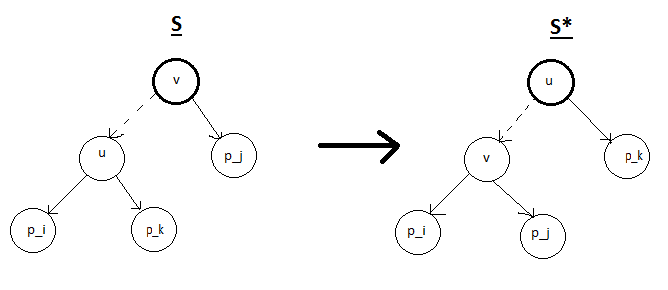
\includegraphics[width=150mm]{q2.png}
	\end{figure}
	
	From the above figure, we can see that $p_k$ is sibling of $p_i$. Since node $v$ is the lowest
	common ancestor of $p_i$ and $p_j$, $h(v)\leq d(p_i,\ p_j)$. For each node $u$ in $Subtree(v)$,
	$h(u)\leq h(v)$. As $d(p_i,\ p_j)$ is the minimum distance, therefore each $h(u)=h(v)$ for an 
	optimal solution.\\
	To obtain $S^*$ from $S$, we swap node $p_k$ and $p_j$.
	\begin{itemize}
		\item \underline{\textbf{Consistent with $d$-}} $S^*$ is consistent as for each internal
		node $u$ in $Subtree(v)$, $h(u)\leq h(v)\leq d(p_i,\ p_j)$. From our assumption, 
		$d(p_i,\ p_j)$ is minimum. Therefore, for any two leaf nodes($x,\ y$) in $Subtree(v)$ in $S^*$,
		their lowest common ancestor($z$) will lie in this $subtree$ only and $h(z)\leq d(p_i,\ p_j)
		\leq d(x,\ y)$.
		\item \underline{\textbf{Optimal Solution-}} As the original solution $S$ was optimal, $i.e.,$
		if $\tau'$ is any other hierarchical metric consistent with $d$, then $\tau'(p_i,\ p_j) \leq 
		\tau(p_i,\ p_j)$ for each pair of points($p_i,\ p_j$), and for all $u$ in $Subtree(v)$, 
		$h(u)\leq h(v)$, and as we can see in $S^*$, $\tau$ is as good as $\tau$ in $S$.
	\end{itemize}
	\subsubsection{Proof of Correctness}
	Let $A$ be the set of with $n$ points and $d(p_i,\ p_j)$ as the minimum distance and
	\begin{center}	 
	\abs{$Opt(A')$} = \abs{$Opt(A)$} - 1, 
	\end{center}
	where $A'$ is the set of points where ($p_i,\ p_j$) are 
	replaced by a single point $p'$.\\\\
	\textbf{\underline{Claim:} Opt($A$) = Opt($A'$) $\cup$ \{node with $\tau(p_i,\ p_j)$\}.}
	
	\begin{itemize}
		\item Opt(\textbf{$A$}) $\geq$ Opt(\textbf{$A'$}) $\cup$ \{node with $\tau(p_i,\ p_j)$\}
		\begin{itemize}
			\item
			A solution for $A$ can be obtained from $A'$, by extending leaf node $p'$ to include 
			points $p_i$, $p_j$ as its children nodes, and $h(p')$ = $d(p_i,\ p_j)$. Therefore,
			for an optimal solution, Opt($A$),\\
			\begin{center}
				Opt(\textbf{$A$}) $\geq$ Opt(\textbf{$A'$}) $\cup$ \{node with $\tau(p_i,\ p_j)$\}
			\end{center}
		\end{itemize}

		\item Opt(\textbf{$A'$}) $\geq$ Opt(\textbf{$A$}) - \{node with $\tau(p_i,\ p_j)$\}
		\begin{itemize}
			\item
			From lemma proved above, there exists an optimal solution for $A$, such that 
			points($p_i,\ p_j$) with minimum distance are siblings in their corresponding binary tree.
			To obtain a solution for $A'$, we replace the leaf nodes $p_i$ and $p_j$ from the optimal
			solution of $A$ with some point $p'$. Therefore, for an optimal solution, Opt($A'$),
			\begin{center}
				Opt(\textbf{$A'$}) $\geq$ Opt(\textbf{$A$}) - \{node with $\tau(p_i,\ p_j)$\}
			\end{center}
		\end{itemize}
		
		From the above two cases, it is clear that :
	\end{itemize}
	\begin{center}
		Opt(\textbf{$A$}) = Opt(\textbf{$A'$}) $\cup$ \{node with $\tau(p_i,\ p_j)$\}.
	\end{center}
\end{document}